\documentclass[11pt,letterpaper]{article}
\usepackage[lmargin=1in,rmargin=1in,tmargin=1in,bmargin=1in]{geometry}
\usepackage{../style/homework}
\usepackage{../style/commands}
\setbool{quotetype}{false} % True: Side; False: Under
\setbool{hideans}{false} % Student: True; Instructor: False

% -------------------
% Content
% -------------------
\begin{document}

\homework{12: Due 11/05}{Science and everyday life cannot and should not be separated.}{Rosalind Franklin}

% Problem 1
\problem{10} Use the quadratic formula to factor $x^2 - 6x - 3$. Show all your work. \pspace

\sol We have\dots \pspace
	\[
	\begin{aligned}
	x&= \dfrac{-b \pm \sqrt{b^2 - 4ac}}{2a} \\[0.3cm]
	x&= \dfrac{-(-6) \pm \sqrt{(-6)^2 - 4(1)(-3)}}{2(1)} \\[0.3cm]
	x&= \dfrac{6 \pm \sqrt{36 + 12}}{2} \\[0.3cm]
	x&= \dfrac{6 \pm \sqrt{48}}{2} \\[0.3cm]
	x&= \dfrac{6 \pm \sqrt{16 \cdot 3}}{2} \\[0.3cm]
	x&= \dfrac{6 \pm 4\sqrt{3}}{2} \\[0.3cm]
	x&= 3 \pm 2 \sqrt{3}
	\end{aligned}
	\] \pspace
Observe that $a= 1$. Therefore, the factorization is\dots
	\[
	x^2 - 6x - 3= 1 \cdot \big(x - (3 + 2\sqrt{3}) \big) \big(x - (3 - 2\sqrt{3}) \big)= \big(x - (3 + 2\sqrt{3}) \big) \big(x - (3 - 2\sqrt{3}) \big)
	\]





\newpage





% Problem 2
\problem{10} Use the quadratic formula to factor $x^2 - 6x + 10$. Show all your work. \pspace

\sol We have\dots \pspace
	\[
	\begin{aligned}
	x&= \dfrac{-b \pm \sqrt{b^2 - 4ac}}{2a} \\[0.3cm]
	x&= \dfrac{-(-6) \pm \sqrt{(-6)^2 - 4(1)(10)}}{2(1)} \\[0.3cm]
	x&= \dfrac{6 \pm \sqrt{36 - 40}}{2} \\[0.3cm]
	x&= \dfrac{6 \pm \sqrt{-4}}{2} \\[0.3cm]
	x&= \dfrac{6 \pm 2i}{2} \\[0.3cm]
	x&= 3 \pm i
	\end{aligned}
	\] \pspace
Observe that $a= 1$. Therefore, the factorization is\dots
	\[
	x^2 - 6x + 10= 1 \cdot \big(x - (3 + i) \big) \big(x - (3 - i) \big)= \big(x - (3 + i) \big) \big(x - (3 - i) \big)
	\]





\newpage





% Problem 3
\problem{10} Use the quadratic formula to factor $4x^2 - 8x + 3$. Show all your work. \pspace

\sol We have\dots \pspace
	\[
	\begin{aligned}
	x&= \dfrac{-b \pm \sqrt{b^2 - 4ac}}{2a} \\[0.3cm]
	x&= \dfrac{-(-8) \pm \sqrt{(-8)^2 - 4(4)(3)}}{2(4)} \\[0.3cm]
	x&= \dfrac{8 \pm \sqrt{64 - 48}}{8} \\[0.3cm]
	x&= \dfrac{8 \pm \sqrt{16}}{8} \\[0.3cm]
	x&= \dfrac{8 \pm 4}{8} \\[0.3cm]
	x&= \dfrac{8 + 4}{8}, \enskip \dfrac{8 - 4}{8} \\[0.3cm]
	x&= \dfrac{12}{8}, \enskip \dfrac{4}{8} \\[0.3cm]
	x&= \dfrac{3}{2}, \enskip \dfrac{1}{2}
	\end{aligned}
	\] \pspace
Observe that $a= 4$. Therefore, the factorization is\dots
	\[
	4x^2 - 8x + 3= 4 \left( x - \dfrac{3}{2} \right) \left( x - \dfrac{1}{2} \right)
	\]
Note that this is the same as the normal factorization:
	\[
	\begin{aligned}
	4x^2 - 8x + 3&= 4 \left( x - \dfrac{3}{2} \right) \left( x - \dfrac{1}{2} \right) \\[0.3cm]
	&= 2 \cdot 2 \cdot \left( x - \dfrac{3}{2} \right) \left( x - \dfrac{1}{2} \right) \\[0.3cm]
	&= 2 \left( x - \dfrac{3}{2} \right) \cdot 2 \left( x - \dfrac{1}{2} \right) \\[0.3cm]
	&= (2x - 3)(2x - 1)
	\end{aligned}
	\]





\newpage





% Problem 4
\problem{10} Find the $x$-intercepts of the quadratic function $y= x^2 - 11x + 30$. Show all your work. \pspace

\sol The $x$-intercepts correspond to the points where $y= 0$. But then
	\[
	\begin{aligned}
	x^2 - 11x + 30&= 0 \\[0.3cm]
	(x - 5)(x - 6)&= 0
	\end{aligned}
	\]
Then either $x - 5= 0$, i.e. $x= 5$, or $x - 6= 0$, i.e. $x= 6$. Therefore, the $x$-intercepts are $(5, 0)$ and $(6, 0)$. 





\newpage





% Problem 5
\problem{10} Find the $x$-intercepts of the quadratic function $y= x^2 - 6x + 9$. Show all your work. \pspace

\sol The $x$-intercepts correspond to the points where $y= 0$. But then
	\[
	\begin{aligned}
	x^2 - 6x + 9&= 0 \\[0.3cm]
	(x - 3)^2&= 0 
	\end{aligned}
	\]
But then $x - 3= 0$, i.e. $x= 3$. Therefore, the only $x$-intercept is $(3, 0)$.  





\newpage





% Problem 6
\problem{10} Find the $x$-intercepts of the quadratic function $y= 5x^2 - 19x + 12$. Show all your work. \pspace

\sol The $x$-intercepts correspond to the points where $y= 0$. But then
	\[
	\begin{aligned}
	5x^2 - 19x + 12&= 0 \\[0.3cm]
	(5x - 4)(x - 3)&= 0
	\end{aligned}
	\]
Then either $5x - 4= 0$, i.e. $x= \frac{4}{5}$, or $x - 3= 0$, i.e. $x= 3$. Therefore, the $x$-intercepts are $(\frac{4}{5}, 0)$ and $(3, 0)$. 





\newpage





% Problem 7
\problem{10} Plot the function $y= x^2 + 2x - 3$. Your plot should include the vertex, axis of symmetry, $y$-intercept, and $x$-intercepts. Show all your work. 
	\[
	\fbox{
	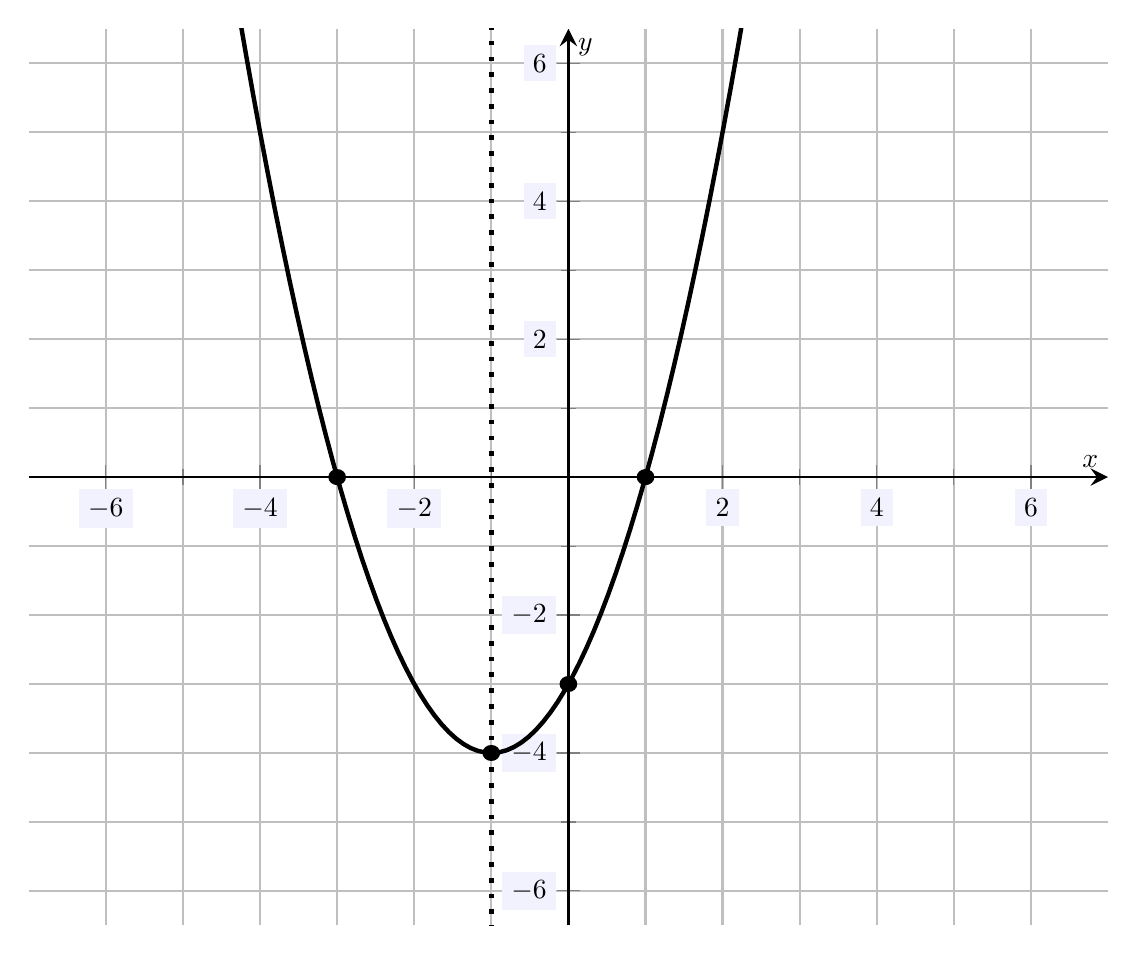
\begin{tikzpicture}[scale=2,every node/.style={scale=0.5}]
	\begin{axis}[
	grid=both,
	axis lines=middle,
	ticklabel style={fill=blue!5!white},
	xmin= -7, xmax=7,
	ymin= -6.5, ymax=6.5,
	xtick={-6,-4,-2,0,2,4,6},
	ytick={-6,-4,-2,0,2,4,6},
	minor tick = {-5,-3,...,5},
	xlabel=\(x\),ylabel=\(y\),
	]
	\addplot[thick, domain= -7:7,samples=150] {x^2 + 2*x - 3};
	\draw[dotted,line width= 0.03cm] (-1,-10) -- (-1,10);
	\draw[fill=black] (-1,-4) circle (0.1);
	\draw[fill=black] (-3,0) circle (0.1);
	\draw[fill=black] (1,0) circle (0.1);
	\draw[fill=black] (0,-3) circle (0.1);
	\end{axis}
	\end{tikzpicture}
	}
	\] \pspace

The $x$-coordinate of the vertex is $x= -\frac{b}{2a}= -\frac{2}{2(1)}= -1$. The $y$-coordinate is then $y(-1)= (-1)^2 + 2(-1) - 3= 1 - 2 - 3= -4$. Therefore, the vertex is $(-1, -4)$. This also means the axis of symmetry is $x= -1$. To find the $x$-intercepts, we solve $x^2 + 2x - 3= 0$. But this implies $(x + 3)(x - 1)= 0$ so that either $x + 3= 0$, i.e. $x= -3$, or $x - 1= 0$, i.e. $x= 1$. Therefore, the $x$-intercepts are $(-3, 0)$ and $(1, 0)$. The $y$-intercept corresponds to the value when $x= 0$. But then $y= 0^2 + 2(0) - 3= -3$. Therefore, the $y$-intercept is $(0, -3)$. 


%\printpoints
\end{document}